\documentclass{article}
\usepackage[utf8]{inputenc}
\usepackage{listings}
\usepackage{graphicx}
\usepackage{float}
\usepackage{xcolor}
\usepackage{geometry}
\usepackage{CJKutf8}
\usepackage{amsmath}
\usepackage{amssymb}

\geometry{a4paper,scale=0.8}
\lstset{
    basicstyle          =   \sffamily,        
    keywordstyle        =   \bfseries,         
    commentstyle        =   \rmfamily\itshape, 
    stringstyle         =   \ttfamily, 
    flexiblecolumns,               
    numbers             =   left,  
    showspaces          =   false, 
    showstringspaces    =   false,
    captionpos          =   t,     
    frame               =   lrtb, 
}

\lstdefinestyle{Python}{
    language        =   Python, % 语言选Python
    basicstyle      =   \zihao{-5}\ttfamily,
    numberstyle     =   \zihao{-5}\ttfamily,
    keywordstyle    =   \color{blue},
    keywordstyle    =   [2] \color{teal},
    stringstyle     =   \color{magenta},
    commentstyle    =   \color{red}\ttfamily,
    breaklines      =   true,  
    columns         =   fixed,  
    basewidth       =   0.5em,
}

\title{\bf\Large  概率论与数理统计 第3次作业}
%%%%%%%%%%%%%%%%%%%%%%%%%%%%%%%%%%%%%%
%% DON'T forget to change this part %%
\author{\bf Name: 宋昊原 \qquad Student ID: 2022010755}
%%%%%%%%%%%%%%%%%%%%%%%%%%%%%%%%%%%%%%

\begin{document}
\begin{CJK}{UTF8}{gbsn}
\maketitle
\section{随机变量的例子}
\subsection{}
有3白2黑共5个球,从中不放回地摸出三个,其中白球的个数为随机变量$X_{1}$.
\\$X_{1}$是离散随机变量
\\将5个球分别标记为1,2,3,4,5,其中1至3为白球,4至5为黑球,则对应的样本空间为
$$ \Omega_{1}=\{(i,j,k)\|i,j,k\in\{1,2,3,4,5\}\land i\neq j \land j\neq k \land i\neq k \} $$
\subsection{}
有一个均匀硬币,连续掷无数次,第一次发生正反面改变(即在此之前的所有试验结果全部相同)的次数为随机变量$X_{2}$.
\\$X_{2}$是离散随机变量
\\对应样本空间$\Omega_{2}$为所有可数长度的“正”“反”串组成的集合.
\subsection{}
在区间(0,1]中随机选取一个实数,所得为$X_{3}$.
$X_{3}$满足下列累积分布函数:
\begin{equation}
    F(x)=\left\{
    \begin{array}{cl}
    0  &  x\leq 0\\
    x & 0<x<1\\
    1  &  x\geq 1\\
    \end{array}\right.
\end{equation}
$X_{3}$为连续随机变量. 对应样本空间为区间(0,1].
\subsection{}
掷五个骰子,规定若没有3个及以上相同的点数,则$X_{4}=0$,否则$X_{4}$等于点数之和.
\\$X_{4}$为离散随机变量. 样本空间$\Omega_{4}$为长度为5的\{1,2,3,4,5,6\}组成的串.
\subsection{}
任取一成年人,其身高构成随机变量$X_{5}$.
\\$X_{5}$可以认为是连续随机变量,样本空间$\Omega_{5}$为世界上所有成年人的集合.
\section{分布函数的性质}
本题需要利用概率的连续性. 故先证明之.
\\\\
\textbf{引理1}\\
设$A_{1}$,$A_{2}$,...为单调递增的事件序列,即$A_{n}\subset A_{n+1}(n=1,2,...)$,令$A=\sum\limits_{n=1}^{\infty}A_{n}$,则$P(A)=\lim_{n\to \infty}P(A_{n})$.
\\\\
\textbf{引理1证明}\\
首先,令$B_{1}=A_{1}$,$B_{n}=A_{n}-A_{n-1}(\forall n\geq 2)$,则有所有$B_{n}(n\geq 1)$两两互斥,且
$$ \forall m,\sum\limits_{n=1}^{m}A_{n}=A_{m}=\sum\limits_{n=1}^{m}B_{n} $$
两边对$m\to \infty$取极限,有
$$ A=\sum\limits_{n=1}^{\infty}A_{n}=\sum\limits_{n=1}^{\infty}B_{n} $$
于是
$$ P(A)=P(\sum\limits_{n=1}^{\infty}B_{n}) $$
由$B_{n}$的互斥性
$$ P(A)=\sum\limits_{n=1}^{\infty}P(B_{n}) $$
$$ =\lim_{m\to \infty}\sum\limits_{n=1}^{m}P(B_{n}) $$
$$ =\lim_{m\to \infty}P(\sum\limits_{n=1}^{m}B_{m}) $$
$$ =\lim_{m\to \infty}P(A_{m}) $$
证毕.
\\\\
\textbf{引理2}\\
设$A_{1}$,$A_{2}$,...为单调递减的事件序列,即$A_{n+1}\subset A_{n}(n=1,2,...)$,令$A=\prod\limits_{n=1}^{\infty}A_{n}$,则$P(A)=\lim_{n\to \infty}P(A_{n})$.
\\\\
\textbf{引理2证明}\\
令$B_{n}=A_{n}^{c},\forall n\in\mathbb{N}$,则\\
$$ B_{n}\subset B_{n+1},\forall n\in\mathbb{N}$$
令$B=\sum\limits_{n=1}^{\infty}B_{n}$\\
$\forall \omega\in A,\forall n\in\mathbb{N},\omega\in A_{n}$,故$\forall n\in\mathbb{N},\omega\notin B_{n}$,故$\omega\notin B$.\\
反之,$\forall \omega\notin A,\exists n_{0}\in\mathbb{N},s.t.\omega\notin A_{n_{0}}$,故$\omega\in B_{n_{0}}$,故$\omega\in B$.\\
于是,$B=A^{c}$.\\
由\textbf{引理1}
$$ P(B)=\lim_{n\to \infty}P(B_{n}) $$
两边同时用1减,则有
$$ P(A)=\lim_{n\to\infty}P(A_{n})$$
证毕.
\subsection{}
定义事件序列
$$ A_{n}=\{\omega\in\Omega|X(\omega)\leq n\} $$
则
$$ \forall n\geq 1, A_{n}\subset A_{n+1} $$
即$A_{n}$满足引理条件,接下来考虑$A=\sum\limits_{n=1}^{\infty}A_{n}$:\\
$\forall \omega\in\Omega,\omega\in A_{\lceil X(\omega)\rceil}$,于是$\omega\in A$.
\\这说明$\Omega\subset A$,故$A=\Omega$.
\\由\textbf{引理1}
$$ \lim_{n\to \infty}P(X\leq n)=P(A)=P(\Omega)=1 $$
于是
$$ \lim_{n\to \infty}F(n)=1 $$
接下来考虑$\lim_{x\to +\infty}F(x)$.
$$\forall\epsilon>0,\exists N\in \mathbb{N},s.t.\forall n>N\land n\in\mathbb{N},|F(n)-1|<\epsilon $$
于是,取$M=N+1$,则$\forall x>M\land x\in\mathbb{R}$,由$F(x)$单调性,有
$$ F(\lfloor x\rfloor)\leq F(x) \leq 1$$
而$\lfloor x\rfloor\geq M>N$,于是
$$ |F(\lfloor x \rfloor)-1|<\epsilon $$
故
$$ |F(x)-1|<\epsilon $$
这说明
$$ \lim_{x\to +\infty}F(x)=1 $$
负无穷处的极限同理可证.
\subsection{}
$\forall x_{0}\in \mathbb{R}$,定义事件序列
$$A_{n}=\{\omega\in\Omega|X(\omega)\leq x_{0}+\frac{1}{n}\} $$
令$A=\{\omega\in\Omega|X(\omega)\leq x_{0}\}$,显然$A\subset A_{n}(\forall n\in\mathbb{N_{+}})$,故$A\subset\prod\limits_{n=1}^{\infty}A_{n}$.\\
假设$\exists\omega\in\prod\limits_{n=1}^{\infty}A_{n}\land\omega\notin A$,则$X(\omega)>x_{0}$,取$n_{0}=\lceil\frac{1}{X(\omega)-x_{0}}\rceil$,则有$\omega\notin A_{n_{0}}$,这与假设矛盾.即上述$\omega$不存在,即$\prod\limits_{n=1}^{\infty}A_{n}\subset A$.\\
故$A=\prod\limits_{n=1}^{\infty}A_{n}$.
由\textbf{引理2},
$$P(A)=\lim_{n\to \infty}P(A_{n})$$
故
$$F(x_{0})=\lim_{n\to\infty}F(x_{0}+\frac{1}{n})$$
接下来考虑$\lim_{x\to x_{0}^{+}}F(x)$.
$$\forall\epsilon>0,\exists N\in \mathbb{N},s.t.\forall n>N\land n\in\mathbb{N},|F(x_{0}+\frac{1}{n})-F(x_{0})|<\epsilon $$
于是,取$\delta=\frac{1}{N+1}$,则$\forall 0\leq x-x_{0}<\delta\land x\in\mathbb{R}$,由$F(x)$单调性,有
$$ F(x_{0}+\frac{1}{\lfloor\frac{1}{x-x_{0}}\rfloor})\geq F(x) \geq F(x_{0})$$
而$\lfloor\frac{1}{x-x_{0}}\rfloor\geq N+1>N$,于是
$$ |F(x_{0}+\frac{1}{\lfloor\frac{1}{x-x_{0}}\rfloor})-F(x_{0})|<\epsilon $$
故
$$ |F(x)-F(x_{0})|<\epsilon $$
这说明
$$ \lim_{x\to x_{0}^{+}}F(x)=F(x_{0}) $$
即$F(x)$在任意$x_{0}\in\mathbb{R}$右侧连续.
\subsection{}
首先证明下述结论:
$$\lim_{x\to a^{-}}F(x)=P(X<a)$$
这仍然可以利用前两问使用的$\epsilon-\delta$语言论述,这里不再赘述,只给出事件序列的构造:
$$A_{n}=\{\omega\in\Omega|X(\omega)<=a-\frac{1}{n}\}$$
$$A=\{\omega\in\Omega|X(\omega)<a\}$$
可以类似地证明,此序列满足\textbf{引理1}条件,故
$$P(x<a)=\lim_{n\to\infty}F(a-\frac{1}{n})$$
利用$F(x)$单调性即可类似地得到
$$P(X<a)=\lim_{x\to a^{-}}F(x)$$
于是
$$P(a\leq X\leq b)=P(X\leq b)-P(x<a)=F(b)-\lim_{x\to a^{-}}F(x)=F(b)-F(a^{-})$$
\section{同分布}
\subsection{}
$$ P(\omega_{1})=P(X=1)=P(Y=2)=\frac{1}{3} $$
$$ P(\omega_{2})=P(X=2)=P(Y=3)=\frac{1}{3} $$
$$ P(\omega_{3})=P(X=3)=P(Y=1)=\frac{1}{3} $$
于是,X和Y均满足对\{1,2,3\}中任何一个取值,概率都为$\frac{1}{3}$,且没有其他可能取值.
\\X和Y同分布.
\subsection{}
列出$X+Y$、$Y-X$的函数关系:
\\\\
\begin{tabular}{l|l|l|l}
	随机变量 & $\omega_{1}$ & $\omega_{2}$ & $\omega_{3}$\\
	\hline
	X+Y & 3 & 5 & 4\\
    \hline
	Y-X & 1 & 1 & -2\\
\end{tabular}
\\\\
于是二者的分布表:
\\\\
\begin{tabular}{l|l|l|l}
	X & 3 & 4 & 5\\
	\hline
	P & $\frac{1}{3}$ & $\frac{1}{3}$ & $\frac{1}{3}$\\
\end{tabular}
\\\\
\begin{tabular}{l|l|l}
	Y & -2 & 1\\
	\hline
	P & $\frac{1}{3}$ & $\frac{2}{3}$\\
\end{tabular}
\section{方差}
\subsection{证明}
$$ Var(X)=\sum\limits_{i}(x_{i}-E(X))^{2}p_{i}$$
$$ =\sum\limits_{i}(x_{i}^{2}p_{i}-2x_{i}E(X)p_{i}+E^{2}(X)p_{i}) $$
$$ =\sum\limits_{i}x_{i}^{2}p_{i}-2E(X)\sum\limits_{i}x_{i}p_{i}+E^{2}(X)\sum\limits_{i}p_{i} $$
$$ =E(X^{2})-2E(X)\times E(X)+E^{2}(X)\times 1 $$
$$ =E(X^{2})-E^{2}(X) $$
\subsection{理解}
中学学过两种方差:数据的方差和随机变量的方差,其中随机变量的方差与课上的定义一致,数据的方差主要差别在于统计一组数据时可以重复,但各个数据的权重均等. 然而,这和随机变量的方差某种程度上还是一回事:
$$ S^{2}=\frac{1}{n}\sum\limits_{i=1}^{n}(x_{i}-\bar{x})^{2} $$
$$ =\frac{1}{n}\sum\limits_{j}n_{j}(x_{j}-\bar{x})^{2} $$
$$ =\sum\limits_{j}\frac{n_{j}}{n}(x_{j}-\bar{x})^{2} $$
$$ =\sum\limits_{j}p_{j}(x_{j}-\bar{x})^{2} $$
这表示,将一组数据的统计方差中相同的元素合并,再将每个元素出现的频率视为选中之的概率,则化为随机变量的方差.
\section{取球问题}
\subsection{不放回版}
假设取球不会停止,设$A_{i}$为第$i$个取出白球,则\\
$$P(X=k)=P(A_{k}|A_{1}^{c}A_{2}^{c}...A_{k-1}^{c})P(A_{1}^{c}A_{2}^{c}...A_{k-1}^{c})$$
$$=\frac{b}{a+b-k+1}\times\frac{a(a-1)...(a-k+2)}{(a+b)(a+b-1)...(a+b-k+2)}$$
$$=\frac{ba!(a+b-k)!}{(a-k+1)!(a+b)!},\forall k=1,2,...,a+1$$
\subsection{放回版}
第一次取出白球出现在第$n$次意味着前面$n-1$次全部取到黑球且第$n$次取到白球,这$n$次互相独立,故
$$P(X=n)=\frac{b}{a+b}\times(\frac{a}{a+b})^{n-1}=\frac{ba^{n-1}}{(a+b)^{n}},\forall n\in\mathbb{N}_{+} $$
此分布相当于成功率$p=\frac{a}{a+b}$的几何分布,直接利用\textbf{第7题}的公式,得
$$ E(X)=\frac{a+b}{a} $$
\section{极端的期望}
存在. 反例如下:
\\\\
样本空间$\Omega=\{\omega_{1},\omega_{2}\}$,两样本点概率分别为0.99和0.01.
\\且有:
$$ X(\omega_{1})=1 $$
$$ X(\omega_{2})=10^{100} $$
$$ Y(\omega_{1})=Y(\omega_{2})=2 $$
于是:
$$ E(X)=1\times 0.99+10^{100}\times 0.01=0.99+10^{98} $$
$$ E(Y)=2 $$
故有
$$ E(X)>100E(Y) $$
然而只要$\omega_{1}$发生,就有$Y>X$,其概率为0.99.
\section{几何分布}
\subsection{分布}
第一次试验成功出现在第$m$次相当于前$m-1$次全部失败而第$m$次成功,其后的情况无所谓. 故
$$ P(X=m)=p(1-p)^{m-1} $$
其中$m$为正整数.
\\$X$的分布表:\\
\begin{tabular}{l|l|l|l|l|l|l}
	X & 1 & 2 & 3 & ... & m & ...\\
	\hline
	P & $p$ & $p(1-p)$ & $p(1-p)^{2}$ & ... & $p(1-p)^{m-1}$ & ...\\
\end{tabular}
\subsection{期望}
$$ E(X)=\sum\limits_{i=1}^{\infty}ip(1-p)^{i-1} $$
$$ =\sum\limits_{i=0}^{\infty}(i+1)p(1-p)^{i} $$
于是
$$ (1-p)E(X)=\sum\limits_{i=1}^{\infty}ip(1-p)^{i} $$
两式相减,有
$$ pE(X)=p+\sum\limits_{i=1}^{\infty}p(1-p)^{i} $$
$$ =p\sum\limits_{i=0}^{\infty}(1-p)^{i} $$
$$ =p\times \frac{1}{1-(1-p)} $$
$$ =1 $$
于是
$$ E(X)=\frac{1}{p} $$
\subsection{方差}
由\textbf{第4题},
$$ Var(X)=E(X^{2})-E^{2}(X) $$
先计算第二项,
$$ E^{2}(X)=\frac{1}{p^{2}} $$
再计算第一项,
$$ E(X^{2})=\sum\limits_{i=1}^{\infty}i^{2}p(1-p)^{i-1} $$
定义函数项级数
$$ f(x)=\sum\limits_{i=1}^{\infty}i^{2}x^{i-1} $$
则
$$ \int_{0}^{x}f(t)dt=\sum\limits_{i=1}^{\infty}ix^{i} $$
$$ \frac{\int_{0}^{x}f(t)dt}{x}=\sum\limits_{i=1}^{\infty}ix^{i-1} $$
$$ \int_{0}^{x}\frac{\int_{0}^{s}f(t)dt}{s}ds=\sum\limits_{i=1}^{\infty}x^{i}=\frac{x}{1-x} $$
于是
$$ f(x)=\frac{d}{dx}(x\frac{d}{dx}(\frac{x}{1-x})) $$
$$=\frac{d}{dx}(\frac{x}{(1-x)^{2}}) $$
$$ =\frac{1+x}{(1-x)^{3}} $$
于是
$$ E(X^{2})=pf(1-p)=p\times\frac{2-p}{p^{3}}=\frac{2-p}{p^{2}} $$
故
$$ Var(X)=E(X^{2})-E^{2}(X)=\frac{1-p}{p^{2}} $$
\section{市场调查}
令$X$为曾通过该平台购买商品的人数,则
$$ X\sim B(25,0.6) $$
以下数据根据二项分布公式经计算机计算得到.
\subsection{}
$$ P(X\geq 15)=0.5858 $$
\subsection{}
$$ P(X>20)=0.0095 $$
\subsection{}
$$ P(X<10)=0.0132 $$
\section{二项分布}
\subsection{期望}
$$ E(X)=\sum\limits_{k=0}^{n}k\tbinom{n}{k}p^{k}(1-p)^{n-k}$$
$$ =0+\sum\limits_{k=1}^{n}\frac{kn!}{k!(n-k)!}p^{k}(1-p)^{n-k}$$
$$ =n\sum\limits_{k=1}^{n}\frac{(n-1)!}{(k-1)!(n-k)!}p^{k}(1-p)^{n-k}$$
$$ =np\sum\limits_{k=1}^{n}\tbinom{n-1}{k-1}p^{k-1}(1-p)^{n-k} $$
$$ =np\sum\limits_{k=0}^{n-1}\tbinom{n-1}{k}p^{k}(1-p)^{n-1-k}$$
$$ =np(p+(1-p))^{n-1}$$
$$ =np$$
\subsection{方差}
$$ Var(X)=E(X^{2})-E^{2}(X) $$
后一项有
$$ E^{2}(X)=n^{2}p^{2} $$
考虑前一项
$$ E(X^{2})=\sum\limits_{k=0}^{n}k^{2}\tbinom{n}{k}p^{k}(1-p)^{n-k}$$
$$ =\sum\limits_{k=1}^{n}\frac{k^{2}n!}{k!(n-k)!}p^{k}(1-p)^{n-k}$$
$$ =np\sum\limits_{k=1}^{n}\frac{k(n-1)!}{(k-1)!(n-k)!}p^{k-1}(1-p)^{n-k}$$
$$ =np\sum\limits_{k=0}^{n-1}\frac{(k+1)(n-1)!}{k!(n-1-k)!}p^{k}(1-p)^{n-1-k}$$
$$ =np\sum\limits_{k=0}^{n-1}\frac{(n-1)!}{k!(n-1-k)!}p^{k}(1-p)^{n-1-k} + np\sum\limits_{k=1}^{n-1}\frac{k(n-1)!}{k!(n-1-k)!}p^{k}(1-p)^{n-1-k}$$
$$ =np+n(n-1)p^{2}\sum\limits_{k=1}^{n-1}\frac{(n-2)!}{(k-1)!(n-1-k)!}p^{k-1}(1-p)^{n-1-k}$$
$$ =np+n(n-1)p^{2}\sum\limits_{k=0}^{n-2}\frac{(n-2)!}{k!(n-2-k)!}p^{k}(1-p)^{n-2-k}$$
$$ =np+n(n-1)p^{2}(p+(1-p))^{n-2}$$
$$ =np+n^{2}p^{2}-np^{2}$$
故
$$ Var(X)=np-np^{2}=np(1-p)$$
\section{标记重捕法}
\subsection{}
总共有$\tbinom{N}{n}$种捞鱼的情形,其中捞到$m$条有记号(即$M$中选$m$同时$N-M$中选$n-m$)的可能共有$\tbinom{M}{m}\tbinom{N-M}{n-m}$种,故
$$ P(X=m)=\frac{\tbinom{M}{m}\tbinom{N-M}{n-m}}{\tbinom{N}{n}}$$
\subsection{}
假定放归后充分混合,且标记并不影响捕捉难易程度,则被捕捞上来的鱼在所有鱼和所有标记鱼两个总体中占比应基本相同(重捕的比例独立于是否有标记),即:
$$\frac{n}{N}=\frac{m}{M}$$
故
$$N=\frac{Mn}{m}$$
\subsection{}
共有$N$条鱼时的概率为
$$ P(X=m)|_{N}=\frac{\tbinom{M}{m}\tbinom{N-M}{n-m}}{\tbinom{N}{n}}=\frac{M!(N-M)!n!(N-n)!}{N!m!(M-m)!(n-m)!(N-M-n+m)!}$$
故
$$ \frac{P(X=m)|_{N+1}}{P(X=m)|_{N}}=\frac{(N-M+1)(N-n+1)}{(N+1)(N-M-n+m+1)}$$
此比值总是正数,下面令此比值大于$1$,有
$$ (N-M+1)(N-n+1)>(N+1)(N-M-n+m+1) $$
$$ N^{2}-(M+n-2)N+(Mn-M-n+1)>N^{2}-(M+n-m-2)N+(-M-n+m+1) $$
$$ mN<Mn-m $$
$$ N<\frac{Mn}{m}-1$$
即,当$N<\frac{Mn}{m}-1$时,$N+1$比$N$概率增加,而$N>\frac{Mn}{m}-1$时,$N+1$比$N$概率减小,而$N=\frac{Mn}{m}-1$和$N=\frac{Mn}{m}$的概率相等.
\\然而考虑到$\frac{Mn}{m}$并不总是整数,不是整数时上述概率表达式没有意义. 使得上述概率最大的$N$应当取区间$[\frac{Mn}{m}-1,\frac{Mn}{m}]$中的整数,即$\lfloor\frac{Mn}{m}\rfloor$.
\\此结果几乎与第二问的估计值相同.
\subsection{}
极大似然估计是在某随机变量的值可以观测确定,但其一个影响因素不可知的情况下,对该影响因素的一种估计策略:认为使得此随机变量取到给定的观测值的概率最高的值就是该影响因素的估计值.
\\\\
我的理解是,在对待估计值的大致分布情况一无所知的情况下,即认为,(至少是概率极大的值附近的)各种可能值都等可能出现,极大似然估计是有道理的. 然而,对某结果的成因的最常见估计策略是贝叶斯公式,假如我们对该待测值的可能分布有一个粗略的估计,例如在某个值附近形成近似的正态分布,即:我们已知各种可能取值的先验概率,那么这种情况下条件概率最大的条件未见得就是最可能的,而应是先验概率与条件概率之积最大(即后验概率最大)的那个值.
\section{计算机实验:二项分布}
\subsection{}
X取15时有最大概率.
\subsection{}
期望值为$\mu=25\times 0.6=15$,即最大概率的X值.
\subsection{}
方差为$\sigma^{2}=25\times 0.6\times 0.4=6$.
\subsection{}
$P(\mu-2\sigma<x<\mu+2\sigma)=P(3<X<27)=1-9.54\times 10^{-7}$.
\subsection{所用代码}
\begin{figure}[htbp]
    \centering
    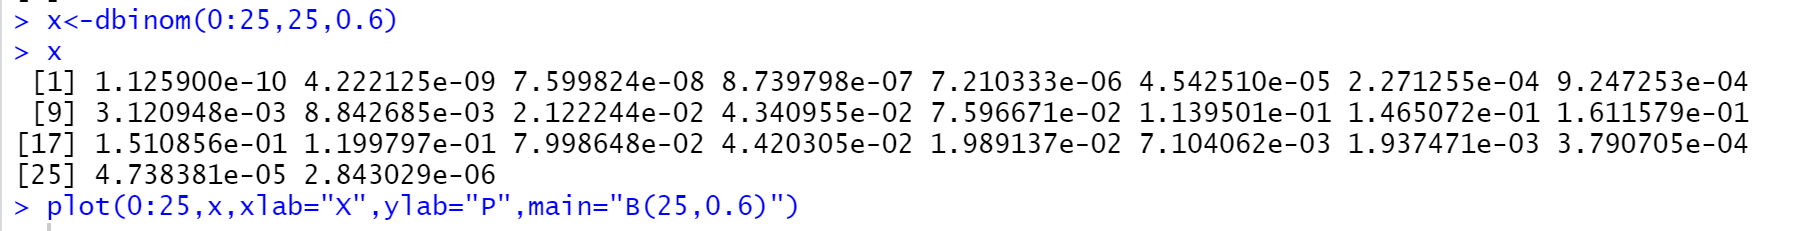
\includegraphics[scale=0.5]{code.png}
\end{figure}
\subsection{分布图}
\begin{figure}[htbp]
    \centering
    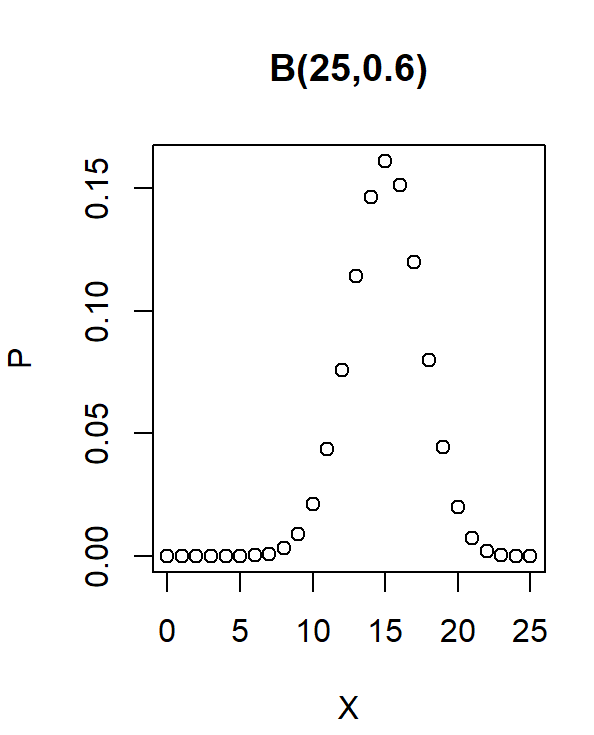
\includegraphics[scale=0.5]{plot.png}
\end{figure}
\end{CJK}
\end{document}